% BHU PYQ -- Professional Exam Template
\documentclass[11pt,a4paper]{article}

\usepackage[a4paper,top=2.5cm,bottom=2.5cm,left=2.8cm,right=2.8cm,headheight=14pt]{geometry}
\usepackage{amsmath,amssymb}
\usepackage[T1]{fontenc}
\usepackage[utf8]{inputenc}
\usepackage{lmodern}
\usepackage{microtype}
\usepackage{fancyhdr}
\usepackage{enumitem}
\usepackage{hyperref}
\usepackage{lastpage}
\usepackage{parskip}
\usepackage{tikz}
\usetikzlibrary{arrows.meta,shapes,positioning}

\hypersetup{colorlinks=true,urlcolor=black,linkcolor=black,
  pdftitle={B.Sc. (Hons.) Zoology Sem-VI ZOB-603 -- BHU PYQ}}

\pagestyle{fancy}
\fancyhf{}
\renewcommand{\headrulewidth}{0.4pt}
\renewcommand{\footrulewidth}{0.4pt}
\fancyhead[L]{\small   \textit{Banaras Hindu University}}
\fancyhead[R]{\small   \textit{Zoology Paper: ZOB-603}}
\fancyfoot[C]{\small Page  \thepage\ of \pageref{LastPage}}


\newlist{parts}{enumerate}{3}
\setlist[parts,1]{label=(\alph*),leftmargin=*,itemsep=4pt,topsep=3pt}
\setlist[parts,2]{label=(\roman*),leftmargin=*,itemsep=2pt,topsep=2pt}
\setlist[parts,3]{label=(\arabic*),leftmargin=*,itemsep=2pt,topsep=2pt}

\newcommand{\pts}[1]{\hfill   \textit{[#1]}}


\begin{document}


\begin{center}
  {\large\bfseries BANARAS HINDU UNIVERSITY}\\[2pt]
  {\normalsize B.Sc. (Hons.) Semester VI Examination, 2022-23}\\[6pt]
  \rule{0.8\linewidth}{0.5pt}\\[6pt]
  {\large\bfseries Zoology}\\[4pt]
  {\large\bfseries Paper: ZOB-603 --- Cell Biology and Genetics}\\[4pt]
  {\normalsize Time: Three hours \hfill Full Marks: 70}
\end{center}

\rule{\linewidth}{0.4pt}

\smallskip



\noindent   \textit{Note: Answer three questions from Section-A (including Question No. 1 which is compulsory) and three questions from Section-B (including Question No. 1 which is compulsory). Use a separate answer book for each section. The figures in the right-hand margin indicate marks.}

\bigskip

\begin{center}
   \textbf{SECTION -- A} \\
   \textbf{(Cell Biology) (Marks: 35)}
\end{center}




\noindent   \textbf{Question 1.} Answer the following parts:

\begin{parts}
  \item Define the importance of:\pts{$3  \times 1 = 3$}
  
\begin{parts}
    \item Polyteny
    \item Telomere
    \item FG-repeats at nuclear pore complex.
  \end{parts}
  
  \item Differentiate between the following:\pts{$2  \times 2 = 4$}
  
\begin{parts}
    \item Tight junction and Gap junction
    \item Integrins and Cadherins.
  \end{parts}

  \item State giving reasons whether the following statements are True or False:\pts{$2  \times 2 = 4$}
  
\begin{parts}
    \item Carrier transporters follow simple Michaelis-Menten kinetics of substrate transport.
    \item Insulin receptors are an example of enzyme-coupled receptors.
  \end{parts}
\end{parts}

\medskip


\noindent   \textbf{Question 2.} Answer the following:

\begin{parts}
  \item What is meant by critical concentration for F-actin polymerization? Explain its role as treadmilling.\pts{6}
  \item Elaborate the different ways through which a cell can be transformed.\pts{6}
\end{parts}

\medskip


\noindent   \textbf{Question 3.} Answer the following:

\begin{parts}
  \item Explain the organization of chromatin and its compaction into metaphase chromosome.\pts{6}
  \item How does SRP regulate co-translational protein transport across ER? In what way is the topology of the membrane-spanning polypeptide maintained during membrane insertion?\pts{6}
\end{parts}

\pagebreak

\medskip


\noindent   \textbf{Question 4.} Answer the following:

\begin{parts}
  \item What are G-proteins? Explain how G-protein signalling is regulated and activates second messengers.\pts{6}
  \item In what way can DNA damage freeze a potentially dividing cell population at the restriction point?\pts{6}
\end{parts}

\bigskip

\begin{center}
   \textbf{SECTION -- B} \\
   \textbf{(Genetics) (Marks: 35)}
\end{center}




\noindent   \textbf{Question 1.} Answer the following parts:

\begin{parts}
  \item Write whether the following statements are True or False giving reasons in 2-3 sentences each:\pts{$3  \times 2 = 6$}
  
\begin{parts}
    \item Regulatory transcription factors bind to core promoter of a gene.
    \item Proteome is larger than genome of a given species.
    \item Tautomeric shifts within the bases that make up the nucleic acids are the most common cause of point mutations.
  \end{parts}
  
  \item What is the status of Lac repressor and CAP protein under the following cellular conditions?\pts{$2  \times 0.5 = 1$}
  
\begin{parts}
    \item Lactose present and glucose absent
    \item Lactose present and glucose present.
  \end{parts}

  \item Distinguish between the following:\pts{$2  \times 2 = 4$}
  
\begin{parts}
    \item First division segregation and Second division segregation in   \textit{Neurospora}
    \item Transposons and Retrotransposons.
  \end{parts}
\end{parts}

\medskip


\noindent   \textbf{Question 2.} Answer the following:

\begin{parts}
  \item What is a `three-point test cross'? Explain how genetic crosses are designed in   \textit{Drosophila} to derive a linkage map of three genes.\pts{4}
  \item Explain how gene regulation occurs via changes in DNA or chromatin structure.\pts{4}
  \item Describe in brief the `general organisation of human genome'.\pts{4}
\end{parts}

\pagebreak

\medskip


\noindent   \textbf{Question 3.} Answer the following:

\begin{parts}
  \item Explain how mutations can be detected using the ClB technique in   \textit{Drosophila}.\pts{4}
  \item How is `trp' operon regulated by attenuation?\pts{4}
  
  
\begin{center}
  
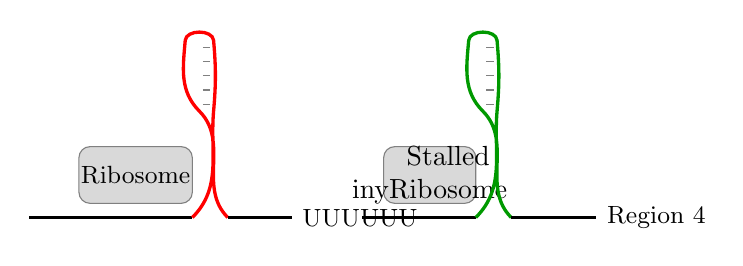
\begin{tikzpicture}[scale=0.9, >=Stealth, every node/.style={font=\small}]
    
\begin{scope}[shift={(0,0)}]
      
ode[above] at (1.2, 3.2) {   \textbf{High Trp (Termination)}};
      \draw[fill=gray!30, draw=gray, rounded corners] (-0.8, 0.2) rectangle (0.8, 1.0) node[pos=0.5] {Ribosome};
      \draw[very thick] (-1.5, 0) -- (0.8, 0);
      
      \draw[very thick, red] (0.8, 0) to[out=45, in=-95] (1.1, 1.5) to[out=85, in=-85] (1.1, 2.5) to[out=95, in=85] (0.7, 2.5) to[out=-95, in=135] (0.9, 1.5) to[out=-45, in=135] (1.3, 0);
      \draw[very thick] (1.3, 0) -- (2.2, 0) node[right] {UUUUUU};
      \foreach \y in {1.6, 1.8, 2.0, 2.2, 2.4} {
        \draw[gray, thin] (0.95, \y) -- (1.05, \y);
      }
      
ode[right, red] at (1.2, 2.0) {3:4 Loop};
    \end{scope}
  
    
\begin{scope}[shift={(5.0,0)}]
      
ode[above] at (1.2, 3.2) {   \textbf{Low Trp (Antitermination)}};
      \draw[fill=gray!30, draw=gray, rounded corners] (-1.5, 0.2) rectangle (-0.2, 1.0) node[pos=0.5, align=center, font= iny] {Stalled\\Ribosome};
      \draw[very thick] (-1.8, 0) -- (-0.2, 0);
      
      \draw[very thick, green!60!black] (-0.2, 0) to[out=45, in=-95] (0.1, 1.5) to[out=85, in=-85] (0.1, 2.5) to[out=95, in=85] (-0.3, 2.5) to[out=-95, in=135] (-0.1, 1.5) to[out=-45, in=135] (0.3, 0);
      \draw[very thick] (0.3, 0) -- (1.5, 0) node[right] {Region 4};
      \foreach \y in {1.6, 1.8, 2.0, 2.2, 2.4} {
        \draw[gray, thin] (-0.05, \y) -- (0.05, \y);
      }
      
ode[right, green!60!black] at (0.2, 2.0) {2:3 Loop};
    \end{scope}
  \end{tikzpicture}
  \end{center}

  \item Describe with the help of a labelled diagram, the sex-determination pathway in human.\pts{4}
  
  
\begin{center}
  
\begin{tikzpicture}[scale=0.85, >=Stealth, every node/.style={font=\small}]
    % Male path
    
ode[draw, fill=blue!10, thick, rounded corners] (xy) at (-3, 3) {XY Chromosomes};
    
ode[draw, fill=blue!10, thick, rounded corners] (sry) at (-3, 1.8) {SRY Gene on Y};
    
ode[draw, fill=blue!20, thick, rounded corners] (gonadM) at (-3, 0.6) {Bipotential Gonad};
    
ode[draw, fill=blue!30, thick, rounded corners] (testis) at (-3, -0.6) {Testes};
    
ode[draw, fill=blue!10, thick, rounded corners] (sertoli) at (-4.2, -1.8) {Sertoli Cells};
    
ode[draw, fill=blue!10, thick, rounded corners] (leydig) at (-1.8, -1.8) {Leydig Cells};
    
ode[draw, fill=blue!15, thick, rounded corners] (amh) at (-4.2, -3.0) {AMH};
    
ode[draw, fill=blue!15, thick, rounded corners] (testo) at (-1.8, -3.0) {Testosterone};
    
ode[draw, fill=blue!40, thick, rounded corners] (male) at (-3, -4.2) {   \textbf{Male Phenotype}};
    
    \draw[->, thick] (xy) -- (sry);
    \draw[->, thick] (sry) -- (gonadM);
    \draw[->, thick] (gonadM) -- (testis);
    \draw[->, thick] (testis) -- (sertoli);
    \draw[->, thick] (testis) -- (leydig);
    \draw[->, thick] (sertoli) -- (amh);
    \draw[->, thick] (leydig) -- (testo);
    \draw[->, thick] (amh) -- (male);
    \draw[->, thick] (testo) -- (male);
  
    % Female path
    
ode[draw, fill=red!10, thick, rounded corners] (xx) at (3, 3) {XX Chromosomes};
    
ode[draw, fill=red!10, thick, rounded corners] (nosry) at (3, 1.8) {No SRY Gene};
    
ode[draw, fill=red!20, thick, rounded corners] (gonadF) at (3, 0.6) {Bipotential Gonad};
    
ode[draw, fill=red!30, thick, rounded corners] (ovary) at (3, -0.6) {Ovaries};
    
ode[draw, fill=red!15, thick, rounded corners] (noamh) at (1.8, -2.2) {No AMH};
    
ode[draw, fill=red!15, thick, rounded corners] (notesto) at (4.2, -2.2) {No Testosterone};
    
ode[draw, fill=red!40, thick, rounded corners] (female) at (3, -4.2) {   \textbf{Female Phenotype}};
    
    \draw[->, thick] (xx) -- (nosry);
    \draw[->, thick] (nosry) -- (gonadF);
    \draw[->, thick] (gonadF) -- (ovary);
    \draw[->, thick] (ovary) -- (noamh);
    \draw[->, thick] (ovary) -- (notesto);
    \draw[->, thick] (noamh) -- (female);
    \draw[->, thick] (notesto) -- (female);
  \end{tikzpicture}
  \end{center}
\end{parts}

\medskip


\noindent   \textbf{Question 4.} Write short notes on the following:\pts{$4  \times 3 = 12$}

\begin{parts}
  \item Ames test
  \item Eukaryotic transcription unit
  
  
\begin{center}
  
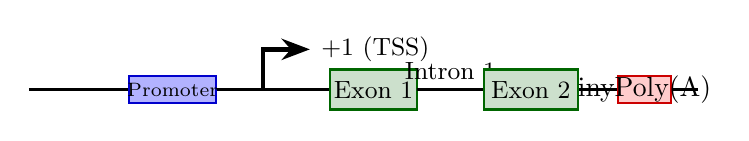
\begin{tikzpicture}[scale=0.85, >=Stealth, every node/.style={font=\small}]
    \draw[thick] (-4, 0) -- (6, 0);
    \draw[fill=blue!30, draw=blue!80!black, thick] (-2.5, -0.2) rectangle (-1.2, 0.2) node[pos=0.5, font=\scriptsize] {Promoter};
    \draw[->, ultra thick, black] (-0.5, 0) -- (-0.5, 0.6) -- (0.2, 0.6) node[right] {+1 (TSS)};
    \draw[fill=green!40!black!20, draw=green!40!black, thick] (0.5, -0.3) rectangle (1.8, 0.3) node[pos=0.5] {Exon 1};
    \draw[thick] (1.8, 0) -- (2.8, 0) node[midway, above] {Intron 1};
    \draw[fill=green!40!black!20, draw=green!40!black, thick] (2.8, -0.3) rectangle (4.2, 0.3) node[pos=0.5] {Exon 2};
    \draw[fill=red!20, draw=red!80!black, thick] (4.8, -0.2) rectangle (5.6, 0.2) node[pos=0.5, font= iny] {Poly(A)};
  \end{tikzpicture}
  \end{center}

  \item Microarray technology
  \item Polygenic inheritance.
\end{parts}

\vfill
\rule{\linewidth}{0.4pt}

\begin{center}\small
\href{https://bhu-exam.vercel.app/}{Click Here}\\[4pt]\href{https://me-aryan.vercel.app/}{Click Here}\\[4pt]\href{https://quashan-me.vercel.app/}{Click Here}
\end{center}

\end{document}
